\section{The JZX Emulator}
The JZX Emulator is the ZX Spectrum emulator implemented in Java. This is the studied emulator and the one we performed some optimizations described below.
Razvan Surdulescu is a Staff software engineer ate Google, graduated from Harvard University and University of Texas at Austin who took the challenge of building a ZX Spectrum emulator written 100\% in Java. This emulator is based on a Linux native emulator called XZX.\\
\indent To emulate the ZX Spectrum, each hardware component must be a logical component made in Java, to correctly simulate the execution. Thus, in our emulator, each Spectrum component is a class that inherits from the abstract class BaseComponent. It is used a composite pattern, where the component BaseSpectrum is the composite, and the other components are the leafs, that allows BaseSpectrum to be the abstraction for all components. The Spectrum components are: BaseSpectrum, BaseMemory, Z80, BaseIO, BaseKeyboard and  BaseScreen.\\
\indent The emulator emulates two different versions of the ZX Spectrum, the 48K model and the 128K. Since the machines are similar, the author made 95\% of the code base shared by the two versions.\\
\indent It does emulate the normal behavior of the ZX Spectrum including the sound and the ROM reading but doesn't emulate the tape reader, because the original uses it to load the and save the software and the emulator uses .z80 files, nor the speaker.
\begin{figure}
	\center{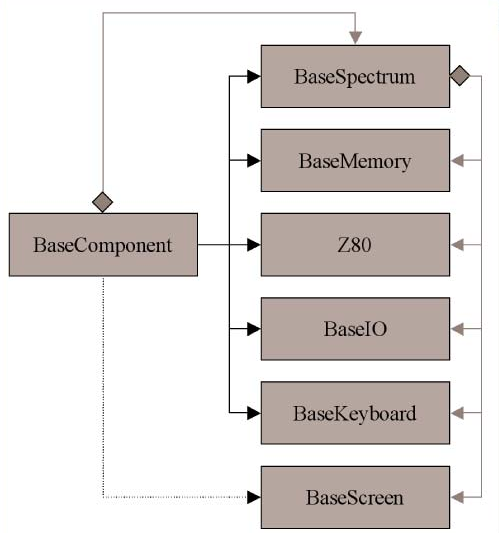
\includegraphics[width=0.4\textwidth]{img/softwareArchitecture.png}}
	\caption{Software architecture.}
\end{figure}

\subsection{CPU Emulation}
The ZX Spectrum emulator is very simple and is based on a decode-and-dispatch interpreter. It maintains the general registers, the program counter, stack pointer and flag registers in memory having an integer variable for each register.
The emulator has a interpretation loop that follows the execution of the program by fetching the memory position pointed by the program counter and then comparing the opcode with all the possible opcodes of the processor in order to discover which instruction should be executed. That comparison is done in a switch case that is not even ordered by the most used instructions.\\
\indent All the code for each instruction is placed inside the respective case statement. This very basic parsing is a major source of inefficiency since for each original instruction the emulator need to perform N comparisons and only then it emulates the instruction. 
Like in the original processor, each time an instruction is executed all the flags are updated. This causes a lot of inefficiency since most of the times the work performed to update the flags is bigger than the work to execute the instruction itself.\\
\indent After fetching and executing an instruction the emulator updates the screen and makes a sleep so that the compatibility with the original processor programs are maintained. The time of the sleep depends on the instruction that has been executed.
Its of main importance that the speed of the spectrum emulator resembles the  speed on the original machine. In the actual case, the host machine is more powerful than the emulated machine and so the main loop of the emulator will  decode and execute instructions at the full speed of the host machine. This is a problem because the normal behavior of the spectrum machine would not be emulated. To solve this issue the emulator maintains a t-state variable that is incremented at the execution of each instruction with a value that depends on the instruction being executed. After executing one instruction in the emulation loop it blocks until a clock thread interrupt is generated. In this way, the clock ensures that although the instructions are decoded at a higher speed than in the original machine, the screen frames and the CPU interrupts are produced at the same rate as the original spectrum hardware.After we have profiled the execution of the emulator code we discovered that the interrupts emulation occupies a great slot of time in the emulation process, and with this i
As you can see the original emulator has lots of inefficiencies and some of them could be reduced by applying techniques learned in the AVE course. In the next section we present some of the possible optimizations.

\subsection{128KB Memory Emulation}
The emulator uses two arrays to emulate the memory of the physical machine. The m\_frame array is the memory visible to the CPU, with only four positions, and the m\_page array its all the available memory that the 128K versions had, with twelve positions. Each position in those arrays has 16KB like the physical pages in the originals had.\\
\indent The first position of the m\_frame its where the ROM pages are loaded. The remaining pages are RAM pages with the same distribution of the original. In the m\_page array, the first four positions are ROM pages and the remaining are RAM pages. This pages are filled with data during the load of the .z80 file.

\subsubsection{Paging}
Like the 128K ZX Spectrum versions do, this emulator is able to do paging too.
The following code takes advantage of a known bug in the original 128K ZX Spectrum. This code activates the second screen, stored in memory at address 7C00h, and writes small files to the RAMdisk causing it to fail in recognizing the existence of the second screen. Type the following code in the 128 BASIC:\\
10 POKE 23388, 24: REM\\
20 FOR I = 1 TO 562\\
30 SAVE! ''F'' + STR\$ I CODE 0, 1\\
40 NEXT I\\
50 PAUSE 0\\
60 POKE 23388, 16: REM\\
RUN\\
\indent As you may noticed, this code begin to fill the screen with colorful squares form bottom to top. If you now type POKE 23388,24: PAUSE 1000 and press enter you will see the screen that the previous chunk of code fill with colorful squares. During the execution of the previous chunk of code the emulator is constantly paging the memory.
